\chapter{Context}

% As of today little work has been done on creating a multihop LoRa Network (see Kris Paper on RPL LoRa in context section)

\section{LoRa\label{section:lora}}

LoRa is a proprietary chirp spread spectrum technology made by Semtech with
integrated Forward Error Correction (FEC).
LoRa operates in this sub-GHz unlicensed Industrial, Scientific and Medical
(ISM) bands.
The main characteristic of LoRa, is that it trades data rate for long range 
and low power consumption with a maximum data rate of 27 kbps~\cite{8030482}.
LoRa supports bi-directional communications with maximum message length of 242
bytes~\cite{loraalliance:lorawanspecification}.

This section will cover the LoRa physical layer parameters, the packet structure and 
will explain how all these parameters influence the Time On Air (ToA).

\subsection{Chirp Spread Spectrum (CSS) modulation}

Chirp Spread Spectrum is a spread spectrum technique, developed in 1940 for
military applications in radars and sonars \cite{semtech:modulationbasics}, but
has been adopted in the recent years for low power data transmission.
Chirps are sinusoidal signals increasing (upchirps) or decreasing (downchirps)
in frequency over time.
Figure~\ref{fig:downchirp} shows an example of a downchirp.

Using CSS has the advantage to ensure equivalent timing and frequency offset
between the receiver and transmitter and robustness to channel degradation
mechanisms (multipath, fading, Doppler, in-band jamming
interference)~\cite{semtech:modulationbasics}.

\tikzset{declare function={f(\x)=sin(540*\x);}}

\begin{figure}[H]
\centering
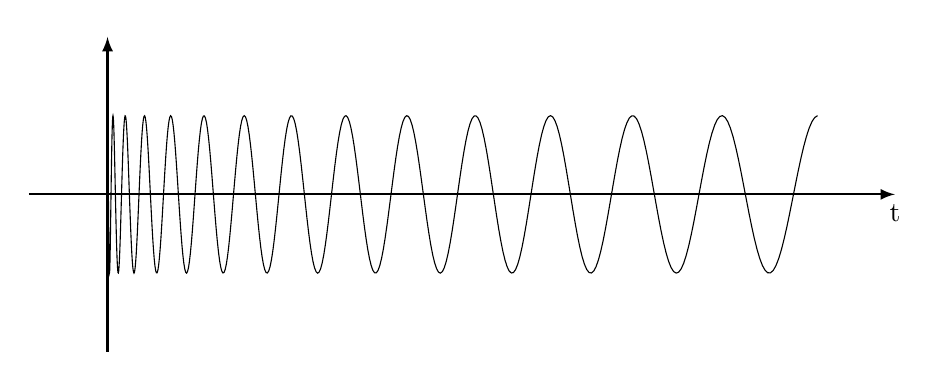
\begin{tikzpicture}
  \draw[thick,-latex] (0,-2) -- (0,2)node[right] {};
  \draw[thick,-latex] (-1,0) -- (10,0)node[below] {t};
  \draw[domain=0.1:9.5,variable=\x,samples=500] plot ({0.10*\x*\x}, {f(\x)});
\end{tikzpicture} 
\caption{Downchirp example\label{fig:downchirp}}
\end{figure}

\subsection{PHY Parameters}

\subsubsection{Spreading Factor (SF)}

The spreading factor, a parameter of the LoRa modulation, represents the
relation~(\ref{eq:sf}) between the symbol rate ($R_{s}$) and chirp rate ($R_{c}$)
(see~\cite{semtech:modemdesign}) where $2^{SF}$ equals to the number of chirps per
symbols.

\begin{equation}
 \label{eq:sf} 
  2^{SF} = \frac{R_s}{R_c}
\end{equation}

The SF can range from 7 to 12, higher SF improve the Signal-to-noise ratio
(SNR) and receiver sensitivity~\cite{semtech:modemdesign}.
Increasing the SF trades transmission range for slower communications.

The LoRa modulation uses orthogonal spreading factors to enable concurrent
packet transmission at the same time with different
spreading factors~\cite{semtech:modulationbasics}.

\subsubsection{Bandwidth (BW)}

Bandwidth is the range of frequencies available during modulation.
LoRa support three bandwidth in the European ISM band.

\begin{itemize}
    \item 125 kHz
    \item 250 kHz
    \item 500 kHz
\end{itemize}

Available bandwidth depends on the region. % See limit of lora wan
% Europe only use 125 and 250 kHz. source needed

The BW is interchangeable with the chirp rate, to do the symbols rate
calculation.
Increasing the BW increases the symbols rate, and thus, the data rate.

\begin{gather}
 \label{eq:bw} 
  BW = R_c (chips/s) \\
  R_s = \frac{BW}{2^{SF}} (symbols / sec)
\end{gather}

According to~\cite{semtech:modulationbasics}, increasing the
bandwidth increases the noise floor (\ref{eq:noisefloorbw}), reducing the
range of the communication.

\begin{equation}
 \label{eq:noisefloorbw} 
  Noise Floor = -174 + 10 \log_{10}(BW)
\end{equation}

% TODO Table with calculation

\begin{table}[h!]
\centering
\begin{tabular}{|c|c|}
\hline
\rowcolor[HTML]{C0C0C0} 
\multicolumn{1}{|c|}{\cellcolor[HTML]{C0C0C0}Bandwidth(kHz)} & Noise Floor (dBm) \\ \hline
125                                                          & -123              \\ \hline
250                                                          & -120              \\ \hline
500                                                          & -117              \\ \hline
\end{tabular}
\caption{Noise floor variation\label{table:bw}}
\end{table}


\subsubsection{Coding-Rate (CR)}

The Coding rate represents the proportion between information bits and error
correction bits. 
Forward Error Correction (FEC) is the process of adding error correction bits to a
transmission, to help with data restoration in case of bit errors.

Increasing the coding rate will decrease the actual data rate. 
There is more overhead, but also more reliability.

The next table~\ref{table:cr} show the CR parameter available in LoRa.

\begin{table}[h!]
\centering
\begin{tabular}{|c|c|}
\hline
\rowcolor[HTML]{C0C0C0} 
  \multicolumn{1}{|c|}{\cellcolor[HTML]{C0C0C0}CR} & Proportion ($\frac{4}{4 + CR}$) \\ \hline
1                                                & $\frac{4}{5}$\\ \hline
2                                                & $\frac{4}{6}$\\ \hline
3                                                & $\frac{4}{7}$\\ \hline
4                                                & $\frac{4}{8}$\\ \hline
\end{tabular}
  \caption{Existing Coding Rates\label{table:cr}}
\end{table}

\subsubsection{Data Rate}

The following equation~\ref{eq:bitrate} calculates the bit rate depending on the
parameters I introduced in the previous sections\cite{semtech:modulationbasics}.

\begin{equation}
 \label{eq:bitrate} 
  R_{b} = SF \frac{\frac{4}{4 + CR}}{\frac{2^{SF}}{BW}} bits/sec
\end{equation}

The data rate can range from $0.3 kbps$ to $27 kbps$ depending on the \emph{SF} % TODO Calculation needed

% TODO datarange table

\subsection{Packet Structure}

This section covers the LoRa packet structure. LoRa employs two packet formats: 
the explicit mode and the implicit mode.
Three part constitute packets.

\begin{itemize}
  \item Preamble
  \item Optional Header
  \item Data payload
\end{itemize}

\begin{figure}[H]
  \centering
\begin{tikzpicture}[
  timeslot/.style={draw, rectangle, minimum size=1cm},
  description/.style={draw, rectangle, minimum size=1cm},
  arr/.style={help lines,black!70,<->},
]
\begin{scope}[xshift=0cm,yshift=0cm,inner sep=0pt, outer sep=0pt]
  \node (desc0) [description, fit={(0,0) (4,2)}, label=center:{Preamble}] {};
  \node (desc1) [description, fit={(4,0) (7,2)}, label=center:{Header}] {};
  \node (desc2) [description, fit={(7,0) (8,2)}, label=center:{CRC}] {};
  \node (desc4) [description, fit={(8,0) (13,2)}, label=center:{Payload}] {};
  \node (desc5) [description, fit={(13,0) (16,2)}, label=center:{Payload CRC}] {};
\end{scope}

\draw[arr]
  ([yshift=12pt]desc1.north west) -- node[fill=white] {$CR = \frac{4}{8}$} ([yshift=12pt]{desc2.north east});
\draw[arr]
  ([yshift=-10pt]desc1.south west) -- node[fill=white] {Explicit mode only} ([yshift=-10pt]{desc2.south east});

\draw[arr]
  ([yshift=12pt]desc4.north west) -- node[fill=white] {$CR$} ([yshift=12pt]{desc5.north east});
\end{tikzpicture}
\caption{LoRa Packet Structure\cite{semtech:sx}\label{fig:packetformat}}
\end{figure}

\begin{description}
  \item[Preamble] synchronize the receiver for the incoming data flow. The
    preamble length is configurable.
  \item[Header] Depends on the packet type explicit or implicit.
  \begin{description}
    \item[Explicit] mode header provides information on the payload.
    \begin{itemize}
      \item Payload length in bytes.
      \item Forward Error Correction code rate.
      \item The presence or not of the payload CRC.
    \end{itemize}
    \item[Implicit] mode removes the header from the packet. This mode should be
      used when payload, coding rate and CRC presence are known and when we want to
      reduce the packet length.
  \end{description}
  \item[Payload] is a variable length field containing the transmitted data as
    well as an optional CRC.
\end{description}

\subsection{Time on Air (ToA)}

The Time on Air is the measure of packet transmission time.
ToA depends on the parameters we introduced previously to count the number of
symbols that constitute each communication of a payload.

The following formula define the duration of each symbol~\ref{eq:tsymlong}.
The equation~\ref{eq:tsym} is equivalent with the relation~\ref{eq:bw}.

\begin{equation}
  \label{eq:tsymlong}
  T_{sym} = \frac{1}{R_{sym}}
\end{equation}

\begin{equation}
  \label{eq:tsym}
  T_{sym} = \frac{2^{SF}}{BW}
\end{equation}

The ToA is the sum of the time to transmit the packet preamble and the packet
payload.

\begin{equation}
  \label{eq:tpacket}
  T_{packet} = T_{preamble} + T_{payload}
\end{equation}

The equation~\ref{eq:tpreamble} calculate the preamble time. The $n_{preamble}$
or preamble length is programmable.

\begin{equation}
  \label{eq:tpreamble}
  T_{preamble} = (n_{preamble} + 4.25)T_{sym}
\end{equation}

The following equation~\ref{eq:payloadsymnb} gives the number of symbols in the
payload of the packet.
The symbols number depend on the following parameters.

\begin{description}
  \item[PL] The payload length in bytes.
  \item[SF] The spreading factor.
  \item[H] Whether (0) or not (1) the header is enabled.
  \item[DE] Whether (1) or not (0) data rate optimization is enabled.
  \item[CR] The coding rate.
\end{description}

\begin{equation}
  \label{eq:payloadsymnb}
  n_{payload} = 8 + \max(ceil(\frac{8PL - 4SF + 28 + 16 - 20H}{4(SF - 2DE)})(CR + 4),0)
\end{equation}

The payload durations in~\ref{eq:tpayload} give the total packet time on air
with~\ref{eq:tpacket}.

\begin{equation}
  \label{eq:tpayload}
  T_{payload} = n_{payload} T_{sym}
\end{equation}


\subsection{Channels}

% See 'Understanding the limits of LoRaWAN' the 3 channels definition in Europe
The channels available is dependant on the country rules we are transmitting from.
The Things Network~\cite{ttnfrequencyplans} did a summary of the available
channels available depending on your frequency plan.

Figure~\ref{fig:channels} presents each LoRaWAN channel available in the
European ISM band (863-870 MHz)~\cite{Polonelli_2019}.

\begin{figure}[H]
  \centering
  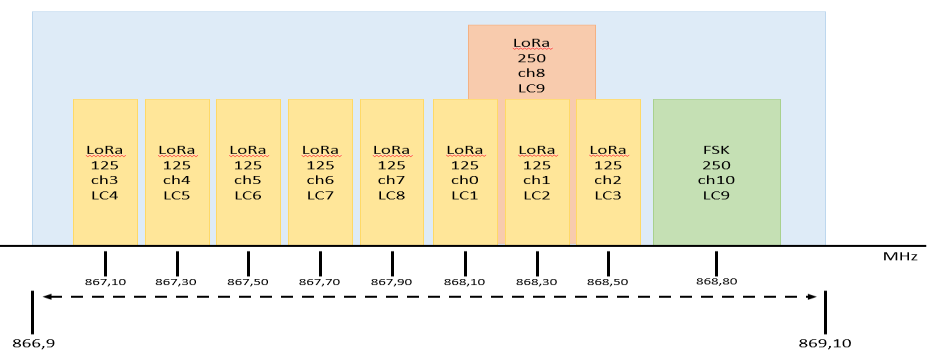
\includegraphics[width=\textwidth]{thesis.tex/chapters/context/fig/channels.png}
  \caption{LoRaWAN Channels in Europe\cite{Polonelli_2019}\label{fig:channels}}
\end{figure}

% TODO Talk about 1% duty cycle

\section{Time-Slotted Channel Hopping (TSCH)}

TSCH is a Medium Access Control (MAC) layer protocol defined by the IEEE
802.15.4 standard~\cite{rfc7554}.
The design inherited from WirelessHART and
ISA100.11a~\cite{Duquennoy2017TSCHA6}.
Time synchronization aim to achieve low power and highly reliable
communications by using the following principles.

\begin{description}
  \item[Time-division multiple access] or (TDMA) by assigning time-slots for each
    participant in the network avoiding collisions.
  \item[Synchronization] time-synchronized nodes syncing their clock with each
    other for being able to keep the notion of time slot.
  \item[Channel Hopping] for better band usage, less interference and more
    throughput.
\end{description}

In the following section I will present the TSCH protocol building blocks.

\subsection{Time Slots}

A time slot in TSCH is a unit of time to execute the network operations. 
The duration of the time slot is not standardized and depend on the physical 
layer we are using. 
Time slots should be long enough for the longest frame size to be sent
between two nodes, together with an acknowledgement~\cite{rfc7554}. 
Every time slot in a TSCH network has the same duration.

For each time slots operations, a schedule orchestrates what each
node of the network will use his time-slot for.

\begin{description}
  \item [Transmit] if a packet is on the outgoing buffer of the node.
  \item [Receive] listen for incoming packets that may arrive.
  \item [Sleep] to save energy.
\end{description}

Each transmitting or receiving time slot is made of the following parts.

\begin{itemize}
  \item The packet transmission or reception.
  \item Guard time for time slots synchronization.
  \item Acknowledgement reception or transmission.
\end{itemize}

\paragraph{}

A set of time slots that repeat over time is known as a slotframe.
A slotframe is made of time slots and empty slots.
The slotframe length has a direct impact on the network capacity.
Figure~\ref{fig:timeslots} represent how time slots and slotframes are
organized together. 

\begin{figure}[H]
  \centering

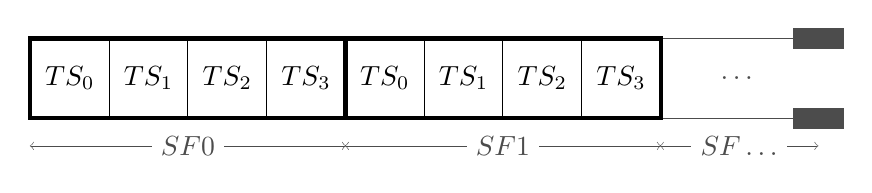
\begin{tikzpicture}[
  timeslot/.style={draw, rectangle, minimum size=1cm},
  arr/.style={help lines,black!70,<->},
]

\foreach [evaluate={\ts=int(mod(\i, 4))}] \i in {0,...,7} {
  \node (ts\i) [timeslot] at (\i, 0) {$TS_{\ts}$};
}
\node (ts8) [minimum height=1cm, minimum width=2cm, black!70] at (8.5, 0) {\ldots};
\draw[help lines, black!70]
  (ts8.north west) -- (ts8.north east) node[fill=white, black!70] {$\ldots$};
\draw[help lines, black!70]
  (ts8.south west) -- (ts8.south east) node[fill=white, black!70] {$\ldots$};

\draw[ultra thick] 
  (ts0.south west) rectangle (ts3.north east)
  (ts4.south west) rectangle (ts7.north east);

\draw[arr]
  ([yshift=-10pt]ts0.south west) -- node[fill=white] {$SF0$} ([yshift=-10pt]{ts3.south east});
\draw[arr]
  ([yshift=-10pt]ts4.south west) -- node[fill=white] {$SF1$} ([yshift=-10pt]{ts7.south east});
\draw[arr]
  ([yshift=-10pt]ts8.south west) -- node[fill=white] {$SF\ldots$} ([yshift=-10pt]{ts8.south east});

\end{tikzpicture}

\caption{Slotframes representation\label{fig:timeslots}}
\end{figure}


\subsection{Absolute Slot Number (ASN)}

The absolute slot number is a shared counter between all the devices that
define the number of time slots elapsed since the start of the start of the
network (see Fig~\ref{fig:asn}).
ASN increases after each time-slot and is calculated with \ref{eq:asn} where $k$
is the slotframe offset.

\begin{equation}
  \label{eq:asn}
  ASN = k SF_{len} + TS_{offset}
\end{equation}

\begin{figure}[H]
\centering
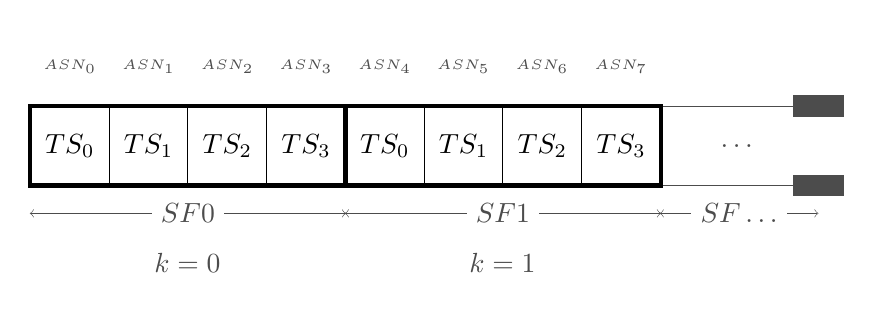
\begin{tikzpicture}[
  asn/.style={black!70, minimum size=1cm},
  timeslot/.style={draw, rectangle, minimum size=1cm},
  arr/.style={help lines,black!70,<->},
  desc/.style={black!70},
]

\foreach \i in {0,...,7} {
  \node (ts\i) [asn] at (\i, 1) {\tiny $ASN_{\i}$};
}
\foreach [evaluate={\ts=int(mod(\i, 4))}] \i in {0,...,7} {
  \node (ts\i) [timeslot] at (\i, 0) {$TS_{\ts}$};
}
\node (ts8) [minimum height=1cm, minimum width=2cm, black!70] at (8.5, 0) {\ldots};
\draw[help lines, black!70]
  (ts8.north west) -- (ts8.north east) node[fill=white, black!70] {$\ldots$};
\draw[help lines, black!70]
  (ts8.south west) -- (ts8.south east) node[fill=white, black!70] {$\ldots$};

\draw[ultra thick] 
  (ts0.south west) rectangle (ts3.north east)
  (ts4.south west) rectangle (ts7.north east);

\draw[arr]
  ([yshift=-10pt]ts0.south west) -- node[fill=white] {$SF0$} ([yshift=-10pt]{ts3.south east});
\draw[arr]
  ([yshift=-10pt]ts4.south west) -- node[fill=white] {$SF1$} ([yshift=-10pt]{ts7.south east});
\draw[arr]
  ([yshift=-10pt]ts8.south west) -- node[fill=white] {$SF\ldots$} ([yshift=-10pt]{ts8.south east});
\node[desc] at
  ([xshift=2cm, yshift=-28pt]ts0.south west) {$k = 0$};
\node[desc] at
  ([xshift=2cm, yshift=-28pt]ts4.south west) {$k = 1$};
\end{tikzpicture}
\caption{Absolute Slot Number\label{fig:asn}}
\end{figure}

\subsection{Channel Hopping}

\emph{Channel Hopping} increases the network capacity with frequency diversity
to mitigate interferences.
Multiple device can share time-slots to transmit at the same time on different
channels.

Links are the conjunction of a time slot and a channel~\cite{Chen2013PerformanceAO}.

\begin{equation}
  \label{eq:links}
  link = (TimeSlot_{number}, Channel_{offset})
\end{equation}

Multiple links constitute a time slot (dependent on the number of channel
available). Devices can transmit on different links during the same time slot.

% TODO Topology example multiple timeslot same time TX on different channels

The channel offset is computed by the transmitter and the receiver with the
function~\ref{eq:channel}. Both node know the $ASN$ and the schedule and can
compute the same channel offset~\cite{rfc7554}.

\begin{equation}
  \label{eq:channel}
  Channel_{offset} = (ASN + Scheduled_{offset}) mod Channel_{number}
\end{equation}

If the slotframe length is a prime number, even with static schedule,
with known channel offset, the timeslot will use a different channel every time.

\subsection{Scheduling}

The TSCH schedule tell each node what to do during a time slot.

Dedicated time slots cell need the following parts to be defined.

\begin{itemize}
  \item Receive or transmit.
  \item The channel offset.
  \item Address of the node to communicate with.
\end{itemize}

Shared cells multiple nodes can transmit at the same time on the same channel.

To ensure the execution of the same slots, each transmission is an opportunity 
for neighbor to resynchronize their clocks.
Synchronization is important to mitigate the nodes internal clock drift.

Time source node send Enhanced Beacon (EB) packet to synchronize the receiving
nodes of the network. When nodes don't resynchronize for a long period of time 
a Keep Alive (KA) is sent and used to adjust the drift at synchronization.

% TODO Graph explaining of we resync like serge did ?

\section{6LoWPAN}

% 6TOP Sublayer

\section{Contiki OS}

Contiki is a free and open source Real-Time operating system (OS) specifically made
for IoT applications. Contiki ships with a low-power IPv6 communication stack
and a variety of routing and MAC protocols making a particularly adapted OS to
use with Wireless Sensor Network (WSN).

Contiki use protothreads, a programming abstraction which around Contiki is
built.
They allow to write event-driven programs with little memory overhead, and
claims to reduce the complexity of embedded programs that used to be written 
like state machines~\cite{10.1145/1182807.1182811}.

The Contiki OS project has been unmaintained since 2017 but at this moment a
fork named Contiki-NG was created.
That fork has been the basis for many LPWAN experimentation with the
development of the 6TiSCH stack for the OS~\cite{Duquennoy2017TSCHA6}.

\paragraph{}

Contiki's Network Protocol stack, also known as \lstinline{NETSTACK}, define
the network stack we are using in a program.
It defines the different OSI layers implementations we 
want to use in a Contiki project (Fig~\ref{fig:netstack}).

NETSTACK implementation allow contiki to communicate between layers without 
knowing the specific implementation of the layer we communicate with.
Developers must define the following variable to change the network stack 
in a Contiki project.

\begin{itemize}
  \item NETSTACK\_NETWORK
  \item NETSTACK\_ROUTING
  \item NETSTACK\_MAC
  \item NETSTACK\_RADIO
\end{itemize}

\begin{figure}[H]
\centering
  \begin{tikzpicture}[->,>=stealth',shorten >=1pt,auto,node distance=1.4cm]

  \tikzstyle{comment}=[
    right=2pt,
    font=\small,
    fill=white,
    text=black,
    draw=black,
  ]

  \tikzstyle{every state}=[rectangle,thick,
    draw=black,fill=gray!20,text=black,
    minimum width= 6cm,
    minimum height= 1.20cm
  ]

  \tikzstyle{smallstate}=[rectangle,thick,
    draw=black,fill=gray!10,text=black,
    minimum width= 4cm,
    minimum height= 1.20cm
  ]

  \node[smallstate]         (A)                    {Network Layer};
  \node[smallstate]         (B) [below of=A]       {Routing};
\begin{scope}[on background layer]
  \node[state, fit=(A)(B)] (AB)                 {};
\end{scope}
  \node[state,below=1cm]         (C) [below of=AB]       {MAC Layer};
  \node[state]         (D) [below of=C]       {Physical Layer};

  \node[comment]       at (AB.north west) {Network Layer};
  % \node[comment]       at (C.north west) {MAC Layer};
  % \node[comment]       at (D.north west) {Physical Layer};
  % \path (A) edge [bend right]    node {     } (B)
  %           edge [bend left]     node {     } (C)
  %       (B) edge [bend left]     node {     } (C)
  %           edge                 node {     } (D)
  %       (C) edge [bend left]     node {     } (A)
  %       (D) edge [bend right=85] node {     } (A);
\end{tikzpicture}
\caption{The Contiki's Network Protocol Stack\label{fig:netstack}}
\end{figure}


\section{Related work}

This section will give a state of the art of the research on
multi-hop network for LoRa and TSCH.

\paragraph{}

Work to port TSCH to a new radio protocol has already been done
in~\cite{uwbtsch}.

\paragraph{BLEach}

\paragraph{UWB-TSCH}

Charlier M. in~\cite{uwbtsch} explore what it need to adapt TSCH for the Ultra
Wideband (UWB). 
In a similar way from LoRa UWB don't allow CCA and can not use CSMA for its 
communications.
His work show what it take to adapt TSCH for another radio layer. 
Its also an evaluation of the performance of TSCH outside of 802.15.4.

\paragraph{}

The respective authors of~\cite{DIAS2018424, 8856256}, look at way to extend
the current LoRaWAN MAC protocol to allow multi-hop communications.

\paragraph{Multihop LoRaWAN Extension} Dias J., Grilo A. in \cite{DIAS2018424}
design a routing protocol that can interoperate with LoRaWAN gateways while
using multi-hop communications for nodes out of the range of the gateway.  
The extension uses beacons to achieve time synchronization, but no channel
hopping is used.

\paragraph{Distributed Queueing (DQ) LoRa}

The authors of~\cite{8856256} extend LoRaWAN

% \subsection{RS LoRa}
% [18] in roald similar to lorawan extension
% \subsection{Listen before talk LoRa}
% [17] in roald work

\paragraph{}

Studies on creating a new MAC protocol for multi-hop LoRa communications in a linear
network has been done in~\cite{Abrardo_2019,duong2018}.

\paragraph{Linear Multihop LoRa}

Abrardo A. and Pozzebon A.~\cite{Abrardo_2019} studied the deployment of a
large scale LoRa network to monitor the underground medieval aqueducts of city center 
of Sienna, the \emph{Bottini}.

Because of the large deployment cost induced by the large tunnels, the negative 
aesthetic impact of a wired network and the risk of flooding, made the author
opt for a battery operated wireless network.

They propose a multi-hop solution for Linear Sensor Network (LSN) based on LoRa by
developing their own MAC protocol tailored for LSN scenario.
This custom protocol is built around assigning time slot for each nodes with
a common schedule for adjacent nodes.
This allow neighbor to synchronize their clock and broadcast messages to the
both end of the aqueducts.

% Their solution allowed the connection of the Bottini

\paragraph{Multi-Hop Linear Network Based on LoRa}

Duong T. in~\cite{duong2018} propose a multi-hop protocol for LoRa linear
network. 
His network is made of two periods. The first is the network initialization to
verify sink is joinable and synchronize the nodes to make them join the data
operation perdiod.
Each node transmit in a different timeslot to their parent node, each hop add
their own information to the packet they are relaying until the sink is
reached.
The clock drift is mitigated by synchronizing on the preamble but the receiver
don't acknowledge the reception of the packet, making the network sensible to
interference since it run on a single channel and SF.

\paragraph{}

The following study look at way to create fully functionning multi-hop network
using LoRa without depending on LoRaWAN specifications.

\paragraph{LoRaBlink}

Bor M., Vidler J., Roedig Utz. in \cite{lorablink} propose the LoRaBlink
protocol, designed to support reliable and energy efficient multi-hop
communication.

Each node of the network remain in listening mode until a beacon is received.
The beacons are used for time synchronization of the time slots.
Node transmit to the parent node that relays it the the sink.
There is not scheduling of which node transmit, it can happen that two node 
transmit at the same time.

% Every nodes of the network keep track of their distance to the sink

Also, LoRaBlink use fixed SF, BW and channel. This decrease the overall throughput 
of the network and make it highly sensible to interference.

\paragraph{RPL+LoRa MAC Protocol}

The Authors of~\cite{8115756} from the ETRO lab of VUB, adapted RPL to enable
multihop communications on top of LoRa. The paper present the modifications of
the objective function to take into account the SF when computing best routes

The paper describe a solution for a network of nodes to discover each other. It
use a router sending packets on different spreading factors while the joining
node listen on the spreading factors by starting by the lowest, this way it
pick the fastest spreading factor available.
It also describe a custom MAC protocol, \emph{RLMAC}, to allow multi-hopping
with LoRa. It manage time-slots between node and allow the PHY settings fine
tuning depending on the links.

The protocol proposed focused on having the fastest delivery time with LoRa
communications while increasing the packet delivery rate (PDR).
Reducing the power consumption was not a concern in this paper.


\paragraph{TSCH-over-LoRa}

In the course of my work, a new study from Haubro M., Orfanadis C.,
Oikonomou G. and Fafoutis X.~\cite{tschoverlora} came out on the exact 
same subject as mine. There work studied the feasibility of porting 
TSCH to LoRa in Contiki OS using SX1272.

The authors proved it was possible to adapt TSCH for LoRa by testing their
implementation with a variety of routing protocol and applications.
Their implementation works on a single SF at the time but they tested it using
SF7 and SF10.

To demonstrate the resilience of TSCH to interference even with LoRa, the
authors made a radio jammer that transmit on different channels. Their
experimentation proved no packet were loss when using channel hopping with
LoRa.
